\section{Stakeholder Viewpoint}
\begin{figure}[H]
    \centering
    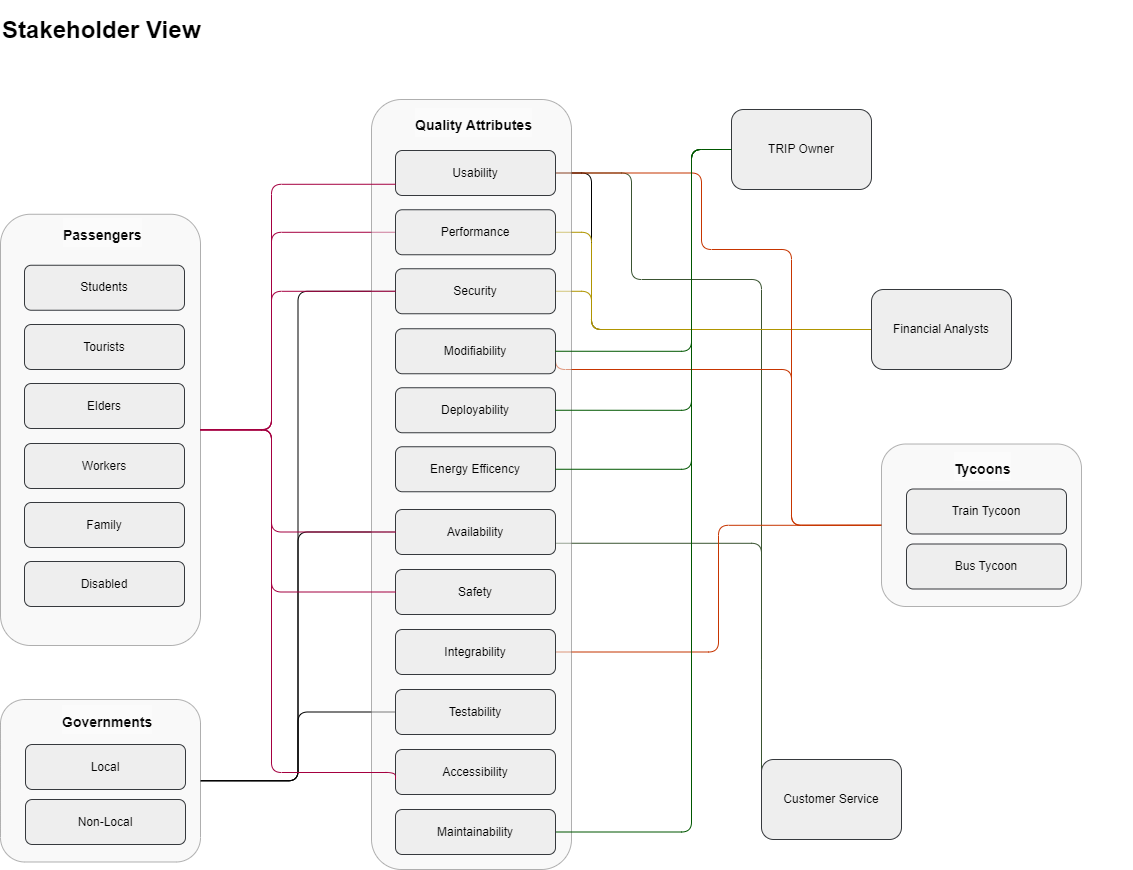
\includegraphics[width=\textwidth]{drawings/views_draft3/stakeholder_view.png}
    \caption{Stakeholder view model.}
    \label{fig:stakeholder_view_model}
\end{figure}

\section{Context Viewpoint}

\begin{figure}[H]
    \centering
    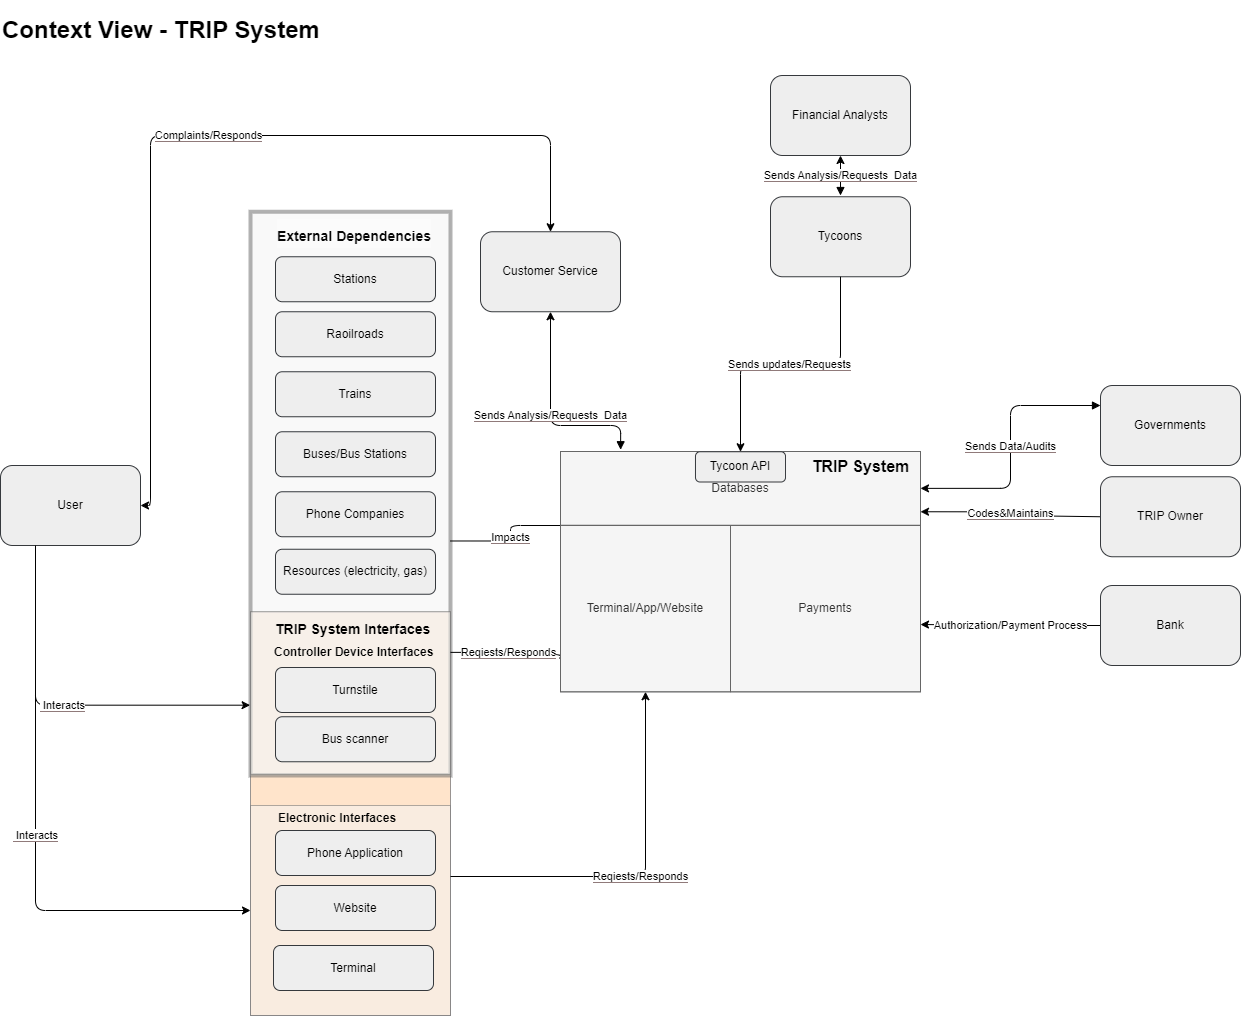
\includegraphics[width=\textwidth]{drawings/views_draft3/context_view.png}
    \caption{Context view model.}
    \label{fig:context_view_model}
\end{figure}

\begin{table}[H]
\centering
\begin{tabular}{@{}clp{9cm}@{}}
\toprule
\textbf{Id} & \textbf{Name} & \textbf{Description} \\
\midrule
1 & User & Individuals who use the TRIP SYSTEM and its associated services, interacting through various interfaces. \\
2 & Customer Service & The department that handles user complaints and feedback, providing support and sending analysis or data requests to the system. \\
3 & Financial Analysts & Experts or entities that review financial data, requiring analytical information from the system for decision-making. \\
4 & Tycoons & The operational decision-makers of the system, possibly managers or algorithms that control system parameters and require data. \\
5 & Tycoon API & The programming interface through which Tycoons receive updates and send requests to the system. \\
6 & TRIP System & The core system that integrates various interfaces and processes, forming the central operation platform. \\
7 & Governments & Regulatory bodies that may require data or perform audits on the system for governance and compliance. \\
8 & TRIP Owner & The entity or person owning and maintaining the TRIP SYSTEM, responsible for its overall functionality. \\
9 & Bank & Financial institution that handles the authorization and processing of payments for the system. \\
10 & Stations & Locations where the TRIP SYSTEM provides service to users, such as train or bus stations. \\
11 & Railroads & Infrastructure providers that offer the tracks on which train services operate. \\
12 & Trains & The vehicles used by the system to transport users from one station to another. \\
13 & Buses/Bus Stations & The bus services and their stations that are part of the transport network. \\
14 & Phone Companies & Telecom service providers that facilitate mobile communication and data transfer for the system. \\
15 & Resources (electricity, gas) & Utility providers that supply essential power and energy required for the system’s operations. \\
16 & Controller Device Interfaces & The interfaces like turnstiles and bus scanners that manage access control and validate user credentials. \\
17 & Electronic Interfaces & Digital platforms such as mobile applications and websites that users interact with for services. \\
\bottomrule
\end{tabular}
\caption{Context view glossary for the TRIP System}
\label{tab:glossary_context_view}
\end{table}


\section{Functional Viewpoint}
\begin{figure}[H]
    \centering
    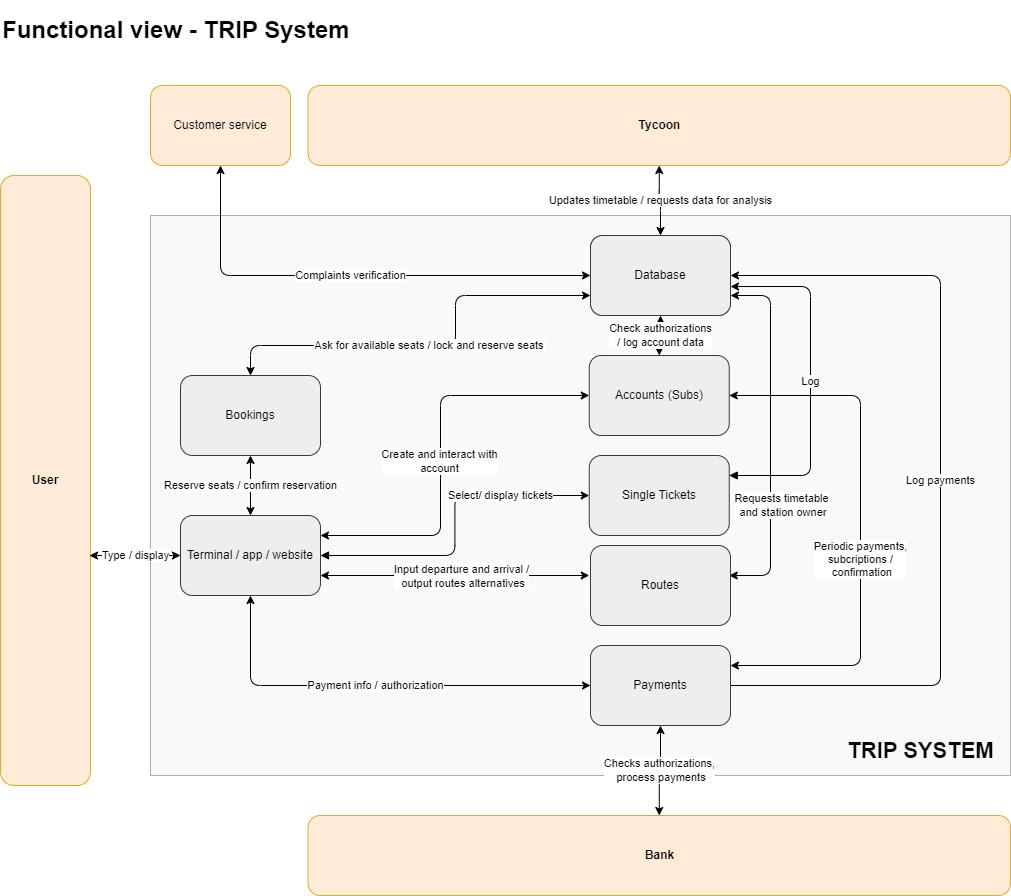
\includegraphics[width=\textwidth]{drawings/views_draft3/functional_view.png}
    \caption{TRIP System.}
    \label{fig:trip_system}
\end{figure}

\begin{table}[H]
    \centering
    \begin{tabular}{@{}clp{9cm}@{}}
    \toprule
    \textbf{Id} & \textbf{Name} & \textbf{Description} \\
    \midrule
    1 & User & End-users of the TRIP SYSTEM who interact with various system components to manage their travel experience. \\
    2 & Customer Service & The interface for users to make inquiries or complaints and receive assistance with bookings or account issues. \\
    3 & Tycoon & The administrative or business logic module that updates timetables and analyzes system data for improvements or reporting. \\
    4 & Database & The central repository that stores all system data including user accounts, bookings, and payment information. \\
    5 & Bookings & The system component where users can inquire about seat availability and make reservations. \\
    6 & Accounts (Subs) & The system managing user accounts and subscriptions, responsible for authorization checks and account data logging. 
    It is is also responsible for single tickets and fillable cards, as they can be seen as temporary and anonymous accounts. \\
    7 & Routes & The component that manages route information and provides users with timetables, station ownership details, and route alternatives. \\
    8 & Payments & The module handling all financial transactions, including user payments and periodic billing. \\
    9 & Bank & The financial institution interface for authorizing and processing payments linked to the system. \\
    10 & Terminal/App/Website & User interfaces through which they can access services such as booking, route information, and payment. \\
    \bottomrule
    \end{tabular}
    \caption{Glossary of elements detailing the components of the TRIP SYSTEM and their roles in facilitating user interaction and service provision.}
    \label{tab:glossary_trip_system}
\end{table}

\begin{figure}[H]
    \centering
    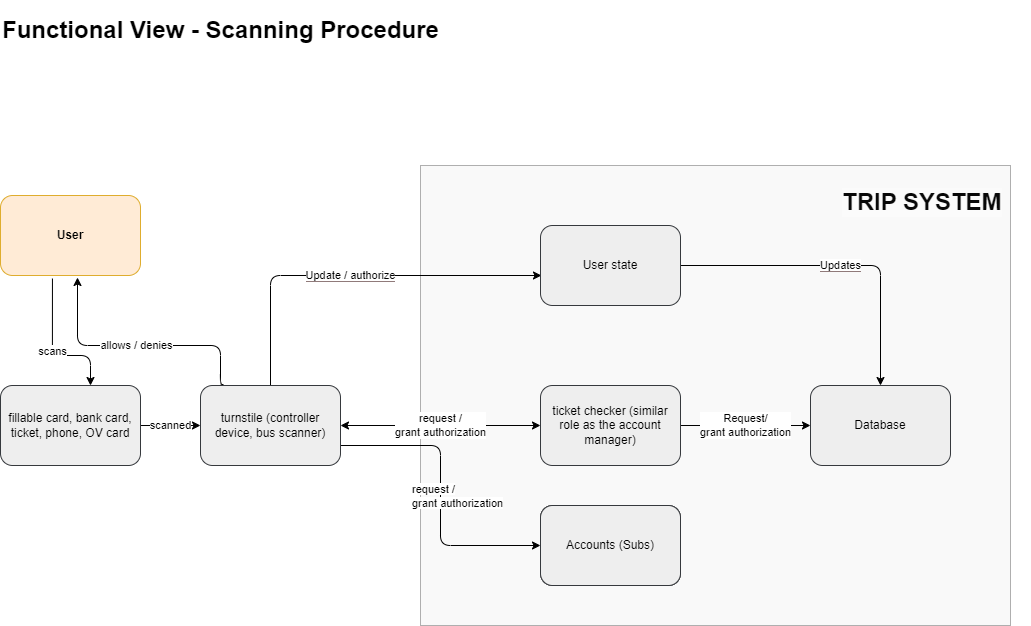
\includegraphics[width=\textwidth]{drawings/views_draft3/functional_view scanning.png}
    \caption{Interaction with a ticket scanner.}
    \label{fig:ticket_scanner}
\end{figure}

\begin{table}[H] % 'H' forces the position here
    \centering
    \begin{tabular}{@{}clp{9cm}@{}} % Adjust the width of the description column as needed to fit the page
    \toprule
    \textbf{Id} & \textbf{Name} & \textbf{Description} \\
    \midrule
    1 & User & The individual who uses the trip system and interacts with various components such as turnstiles and ticket checkers. \\
    2 & Fillable Card, Bank Card, Ticket, Phone, OV Card & Various forms of identification or payment methods that the user can use within the system. These are scanned by the turnstile to allow or deny access. \\
    3 & Turnstile (Controller Device, Bus Scanner) & A physical barrier or scanner that reads the user's ticket or card and determines whether to grant or deny access based on the user state or account information. \\
    4 & User State & A system component that maintains the current state of the user within the system, including authorization and access rights, which is updated upon user interaction with the turnstile. \\
    5 & Ticket Checker (Account Manager) & An agent or system role similar to the account manager that requests or grants authorization for user access, potentially by checking the user state against the database. \\
    6 & Accounts (Subs) & The subsystem managing user accounts and subscriptions, which may interact with the turnstile and ticket checker to verify and update user access rights. \\
    7 & Database & The central storage for the trip system, which records user states, transactions, and account details. It receives updates from various system components and provides information to authorize user access. \\
    \bottomrule
    \end{tabular}
    \caption{Glossary of elements for the Functional View - Turnstiles, detailing the components and their roles in user access and authorization within the TRIP SYSTEM.}
    \label{tab:glossary_turnstiles}
\end{table}

\section*{Information Viewpoint}

\begin{figure}[H]
    \centering
    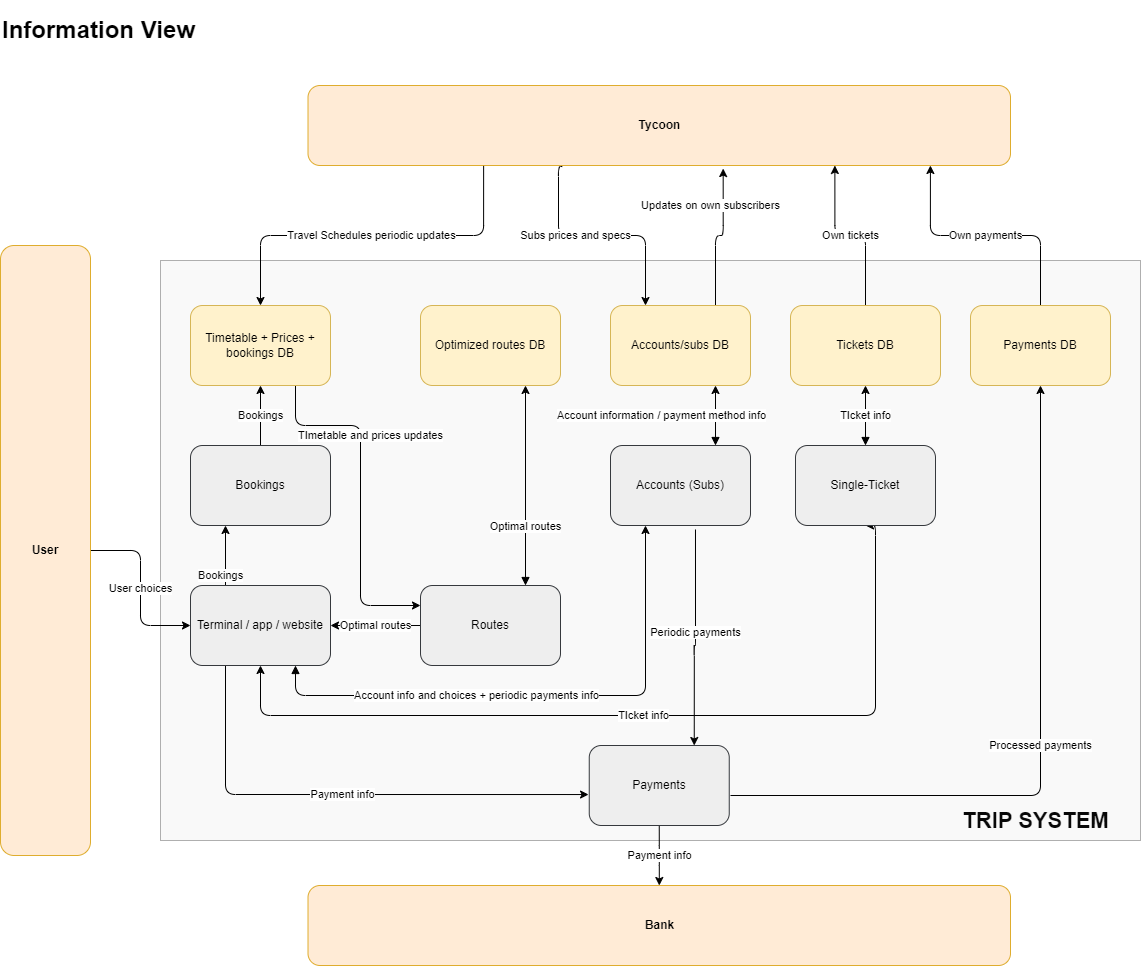
\includegraphics[width=\textwidth]{drawings/views_draft3/information_view.png}
    \caption{Information view.}
    \label{fig:information_view}
\end{figure}
\begin{table}[ht]
\centering
\begin{tabular}{@{}llp{10cm}@{}}
\toprule
\textbf{Id} & \textbf{Name} & \textbf{Description} \\
\midrule
1 & Bookings & Component responsible for managing booking requests and tracking the number of spots left for each train. \\
2 & Tycoon & Module that determines the timetable and prices for specific routes and interacts with the bookings database for updates. \\
3 & Routes & Component that manages route information and calculates prices for the services offered. \\
4 & Accounts (subs) & System managing account and subscription info, handling requests or updates in the accounts/subscribers database. \\
5 & Payments & Component processing payment transactions and handling requests or updates in the payments database. \\
6 & Timetable + Prices + Bookings DB & A database storing timetables, pricing, and current bookings for services. \\
7 & Optimized Routes DB & A database containing the optimized routes cached after being calculated by the Routes Optimization Module. \\
8 & Accounts/Subs DB & A database containing info about the accounts and their subscriptions. \\
9 & Payments DB & A database recording completed payments, accessible for queries such as complaints or refunds. \\
\bottomrule
\end{tabular}
\caption{Glossary of elements for the Functional View - Databases, detailing the components and databases of the TRIP SYSTEM.}
\label{tab:glossary_elements}
\end{table}

\begin{figure}[H]
    \centering
    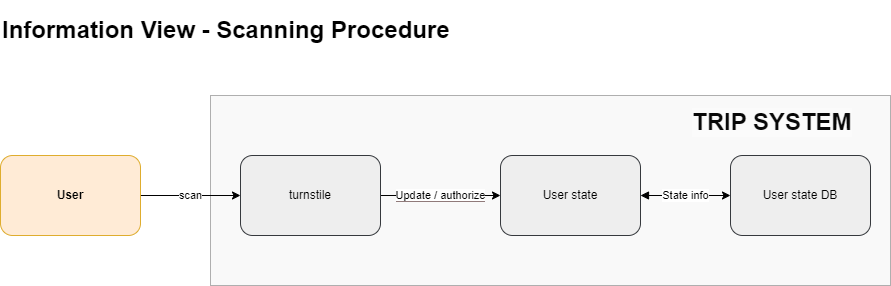
\includegraphics[width=\textwidth]{drawings/views_draft3/information_view scanning.png}
    \caption{Information view related to the scanning procedure.}
    \label{fig:information_view_scanning}
\end{figure}

\section*{Concurrency Viewpoint}

\section*{Development Viewpoint}

\section*{Deployment Viewpoint}